\section{Umsetzung}
Das Architekturbild~\ref{fig:umsetzung_frontendarchitektur_4} auf Seite~\pageref{fig:umsetzung_frontendarchitektur_4}
zeigt die Architektur des Frontends und die Kommunikation mit dem API Connect Service. Dabei sollen sowohl das Frontend
als auch die Smartphone-Apps mit dem API Gateway kommunizieren, um die Anfragen zu vereinheitlichen.

Ein Cloud Foundry-Container wird mit einem Node.js-Boilerplate versehen. Mit Hilfe des Boilerplates lassen sich
Node.js-Applikationen innerhalb des Containerts verwalten und nutzen. Es stellt eine Runtime zur Verfügung, in welcher
das Frontend laufen kann.

Die Smartphone-Apps werden auf Basis von Android und auch iOS entwickelt. Beide Systeme erhalten innerhalb der App ein
WebView-Layout, welche für das Laden und das Darstellen der Webseite zuständig ist. Damit ist es einfach, eine schon
erstellte, responsive Webseite optimal für ein Smartphone zu nutzen. Zusätzlich können Feinheiten wie angepasste Layouts
der einzelnen Systeme übernommen werden.

Die Kommunikation zwischen Frontend und API Connect sowie zwischen den entwickelten Smartphone-Apps und dem API Connect
Service laufen über REST-Aufrufe (englisch REST-Calls).

Da in den Smartphone-Apps lediglich das schon geschriebene Frontend geladen wird, müssen die Aufrufe nur ein Mal
spezifiziert und umgesetzt werden.

\begin{figure}[h]
    \centering
    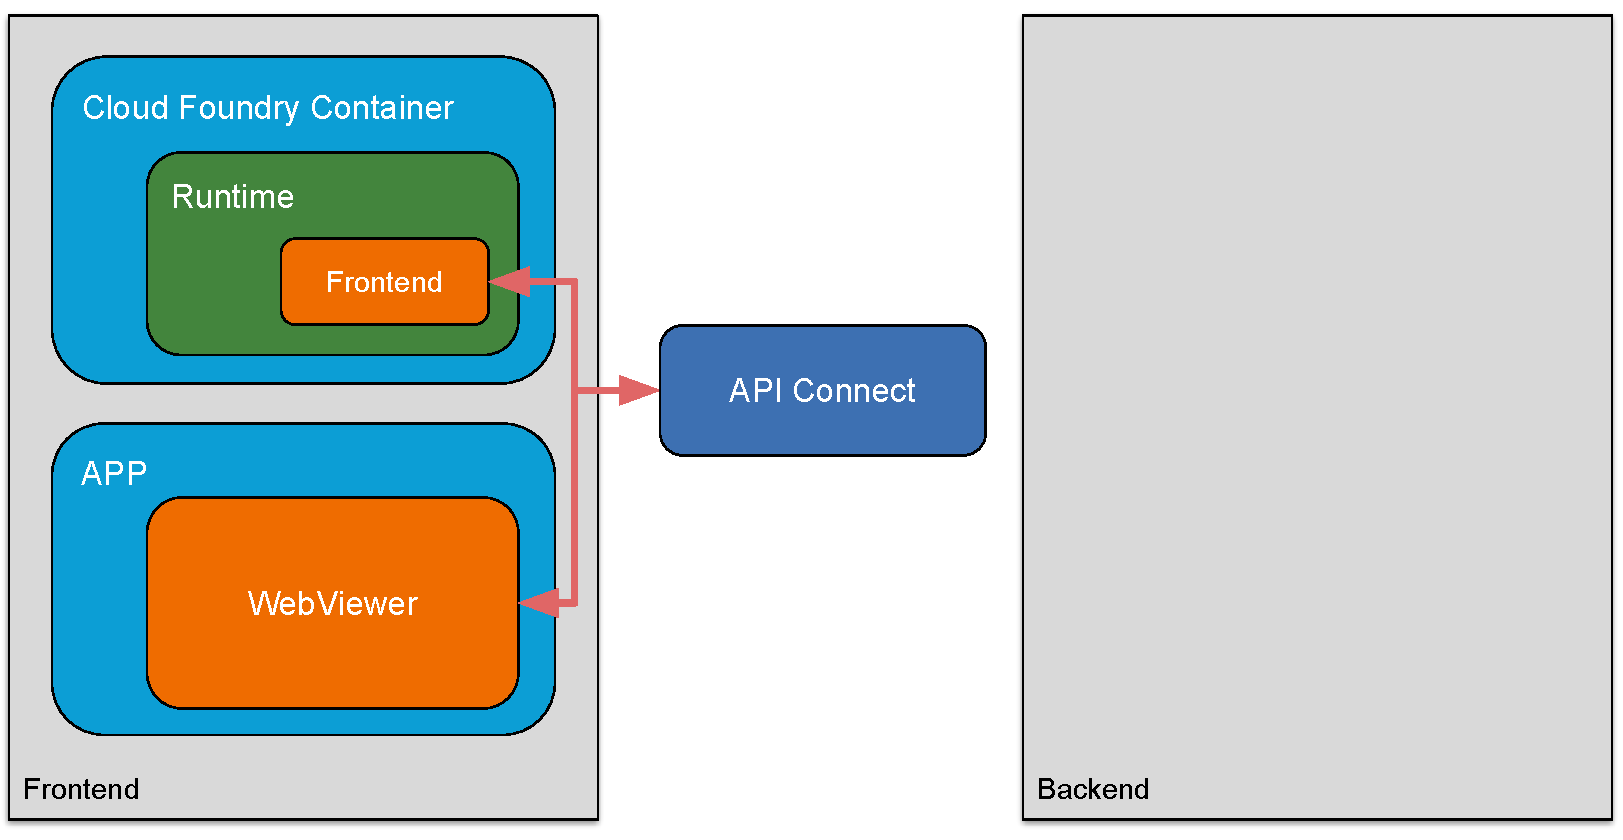
\includegraphics[width=\textwidth]{images/kapitel_4/architektur_frontend.pdf}
    \caption{Übersicht der Zielarchitektur}
    \label{fig:umsetzung_frontendarchitektur_4}
\end{figure}

%% TODO noch schreiben
\subsection{Webseite}
\label{subsec:webseite}
Bauen und erstellen der eigentlichen Webseite
Mockups werden auch erstellt. Wie sehen die aus etc.

\colorbox{yellow}{Hier fehlt was}

%% TODO noch schreiben
\subsubsection{Mockups erstellen}
\colorbox{yellow}{Hier fehlt was}

\begin{figure}[h]
    \centering
    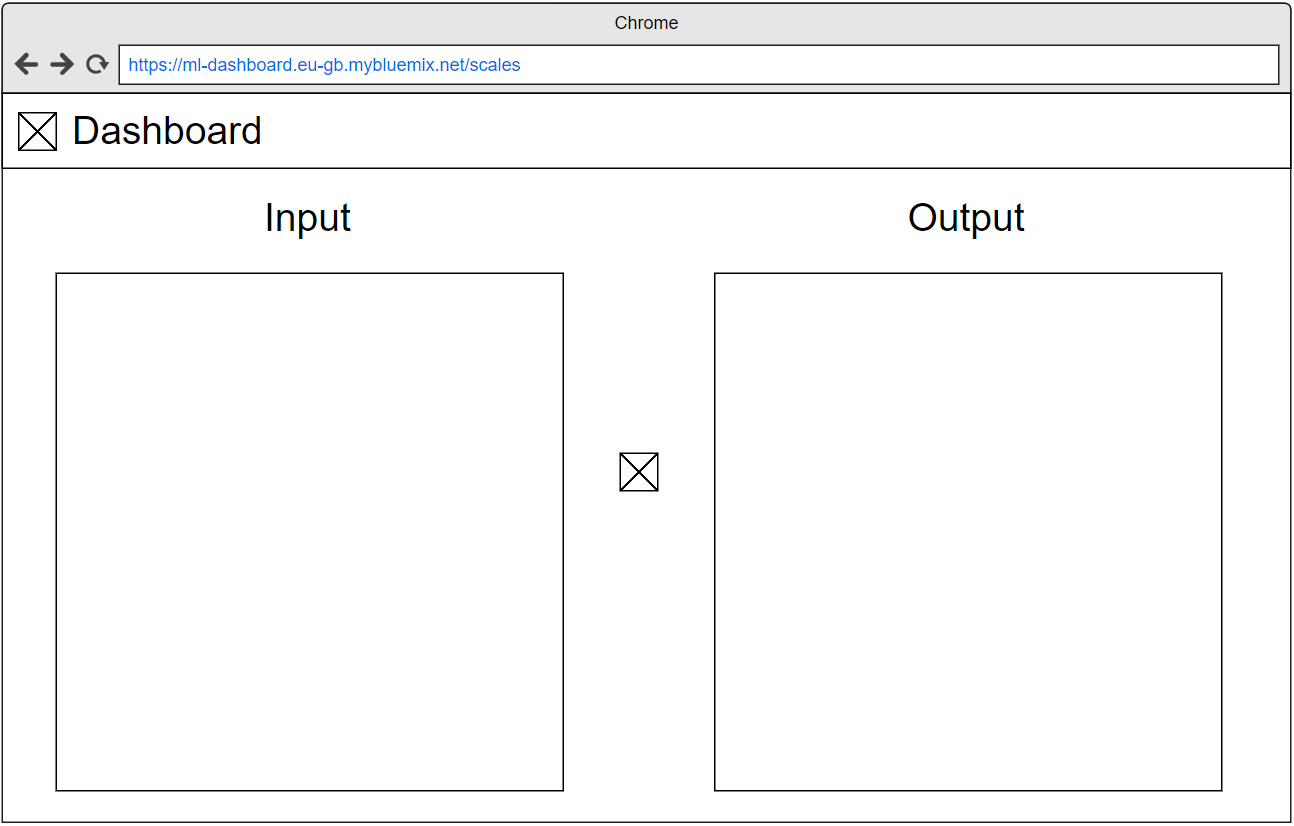
\includegraphics[width=\textwidth]{images/kapitel_4/mockup_scale_1.png}
    \caption{Erstes Mockup für das Dashboard}
    \label{fig:umsetzung_mockup_scale_1}
\end{figure}

\begin{figure}[h]
    \centering
    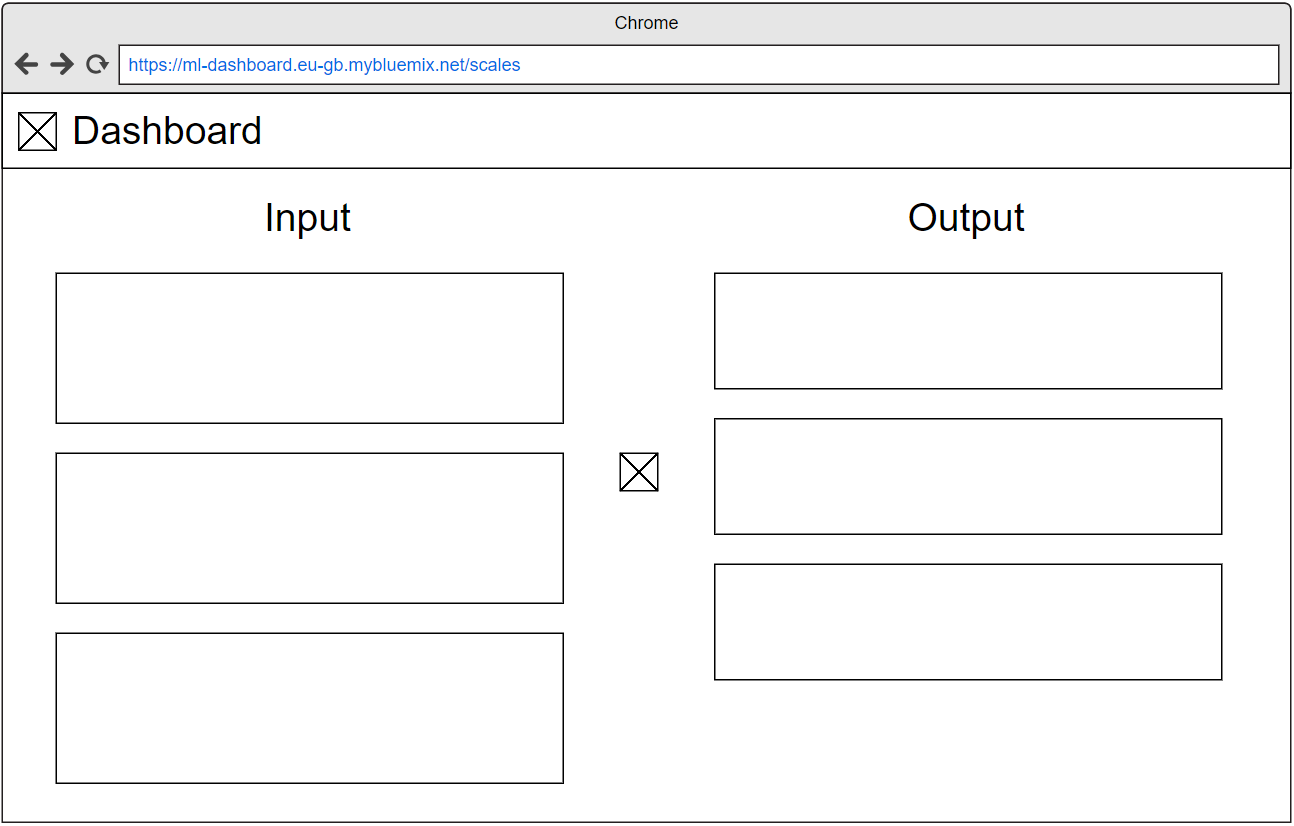
\includegraphics[width=\textwidth]{images/kapitel_4/mockup_scale_2.png}
    \caption{Überarbeitetes Mockup für das Dashboard}
    \label{fig:umsetzung_mockup_scale_2}
\end{figure}

\begin{figure}[h]
    \centering
    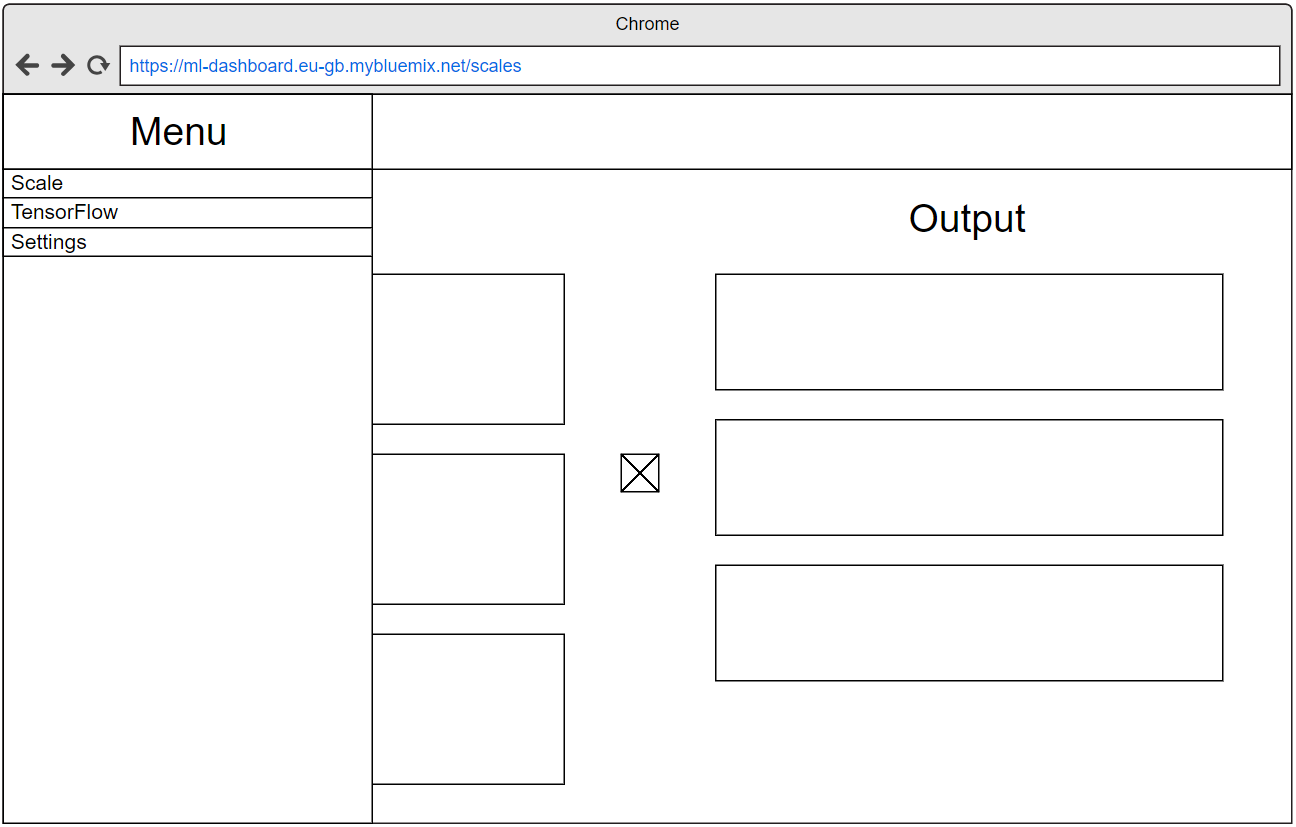
\includegraphics[width=\textwidth]{images/kapitel_4/mockup_scale_menu.png}
    \caption{Mockup für die Navigation}
    \label{fig:umsetzung_mockup_scale_menu}
\end{figure}

\begin{figure}[h]
    \centering
    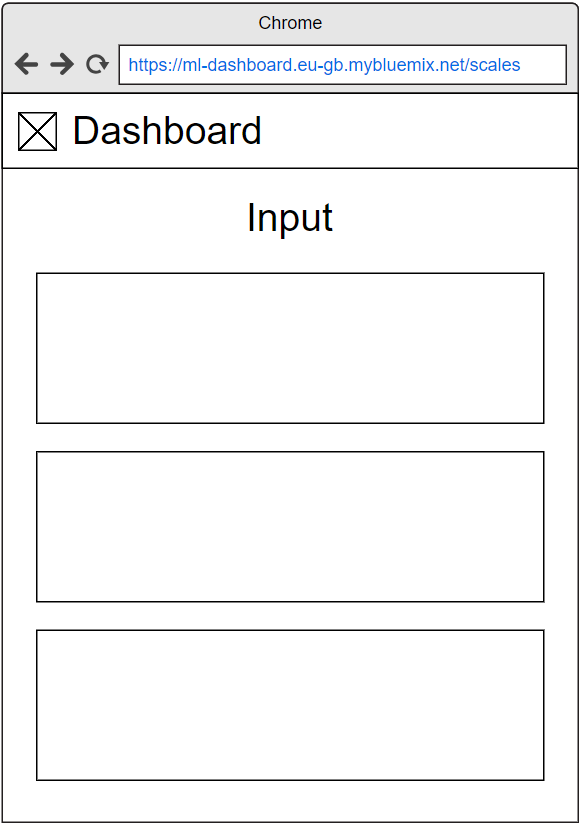
\includegraphics[scale=0.5]{images/kapitel_4/mockup_scale_responsive.png}
    \caption{Mockup des responsiven Designs}
    \label{fig:umsetzung_mockup_scale_responsive}
\end{figure}

%% TODO noch schreiben
\subsubsection{Gedanken zu Responsive}
Wir wollen ja auch Smartphones bedienen. Was muss man beachten? Was habe ich mir gedacht? Was wurde nun daraus?
Eventuell auch mit Mockups belegen.
\colorbox{yellow}{Hier fehlt was}

%% TODO noch schreiben
\subsubsection{Webseite umsetzen}
\colorbox{yellow}{Hier fehlt was}

\begin{figure}[h]
    \centering
    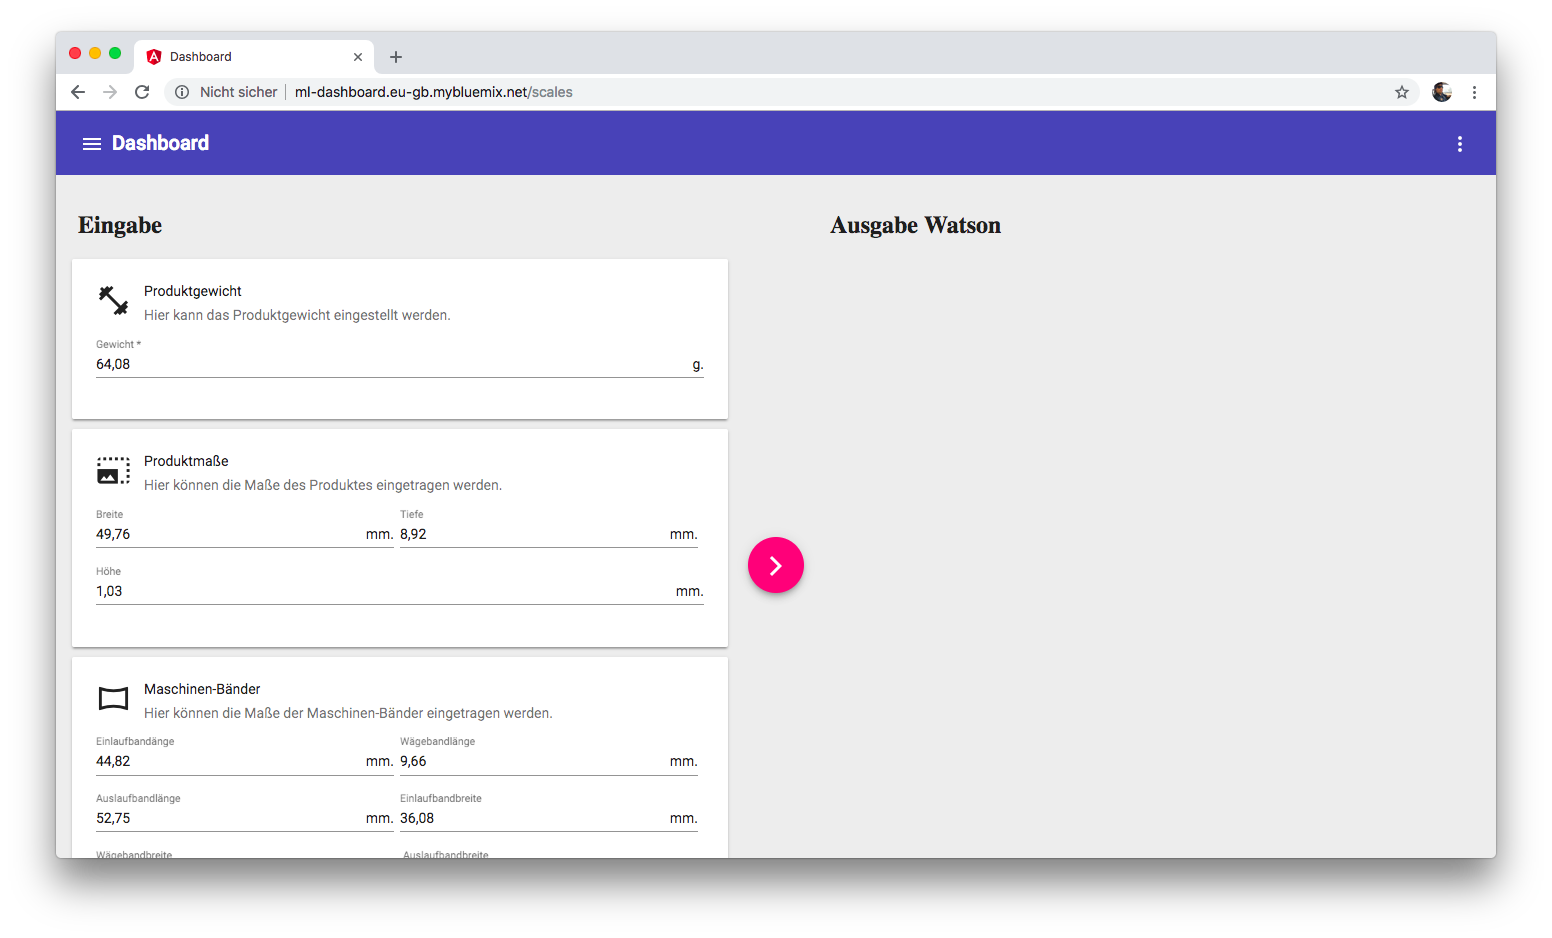
\includegraphics[width=\textwidth]{images/kapitel_4/website_input.png}
    \caption{Kompletter Model flow}
    \label{fig:umsetzung_website_input}
\end{figure}

\begin{figure}[h]
    \centering
    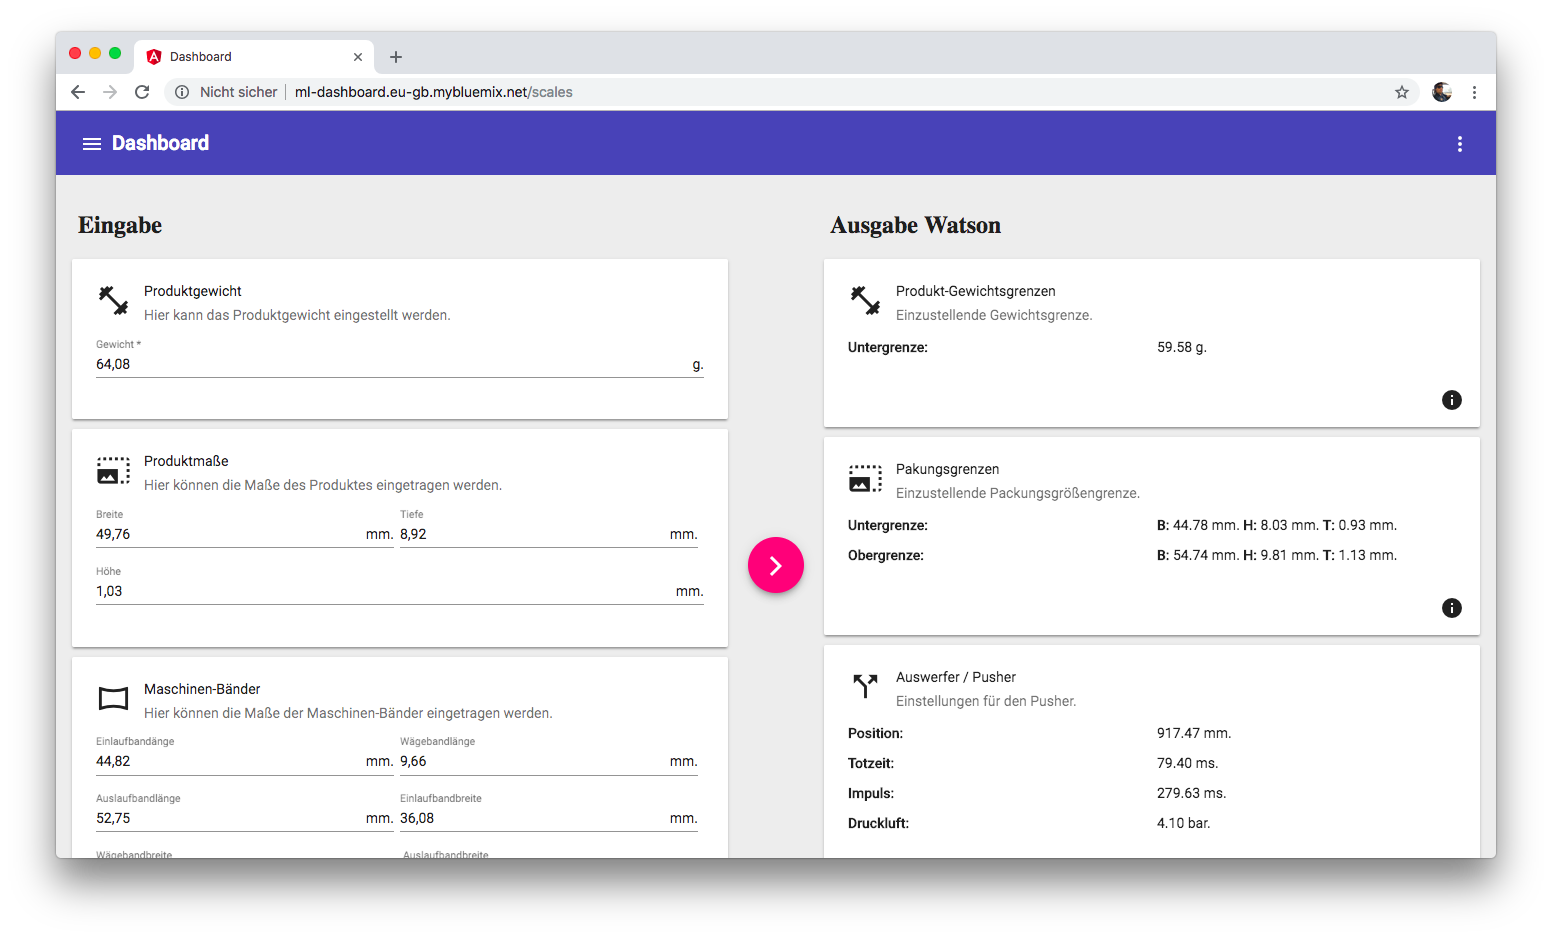
\includegraphics[width=\textwidth]{images/kapitel_4/website_output.png}
    \caption{Kompletter Model flow}
    \label{fig:umsetzung_website_output}
\end{figure}

\begin{figure}[h]
    \centering
    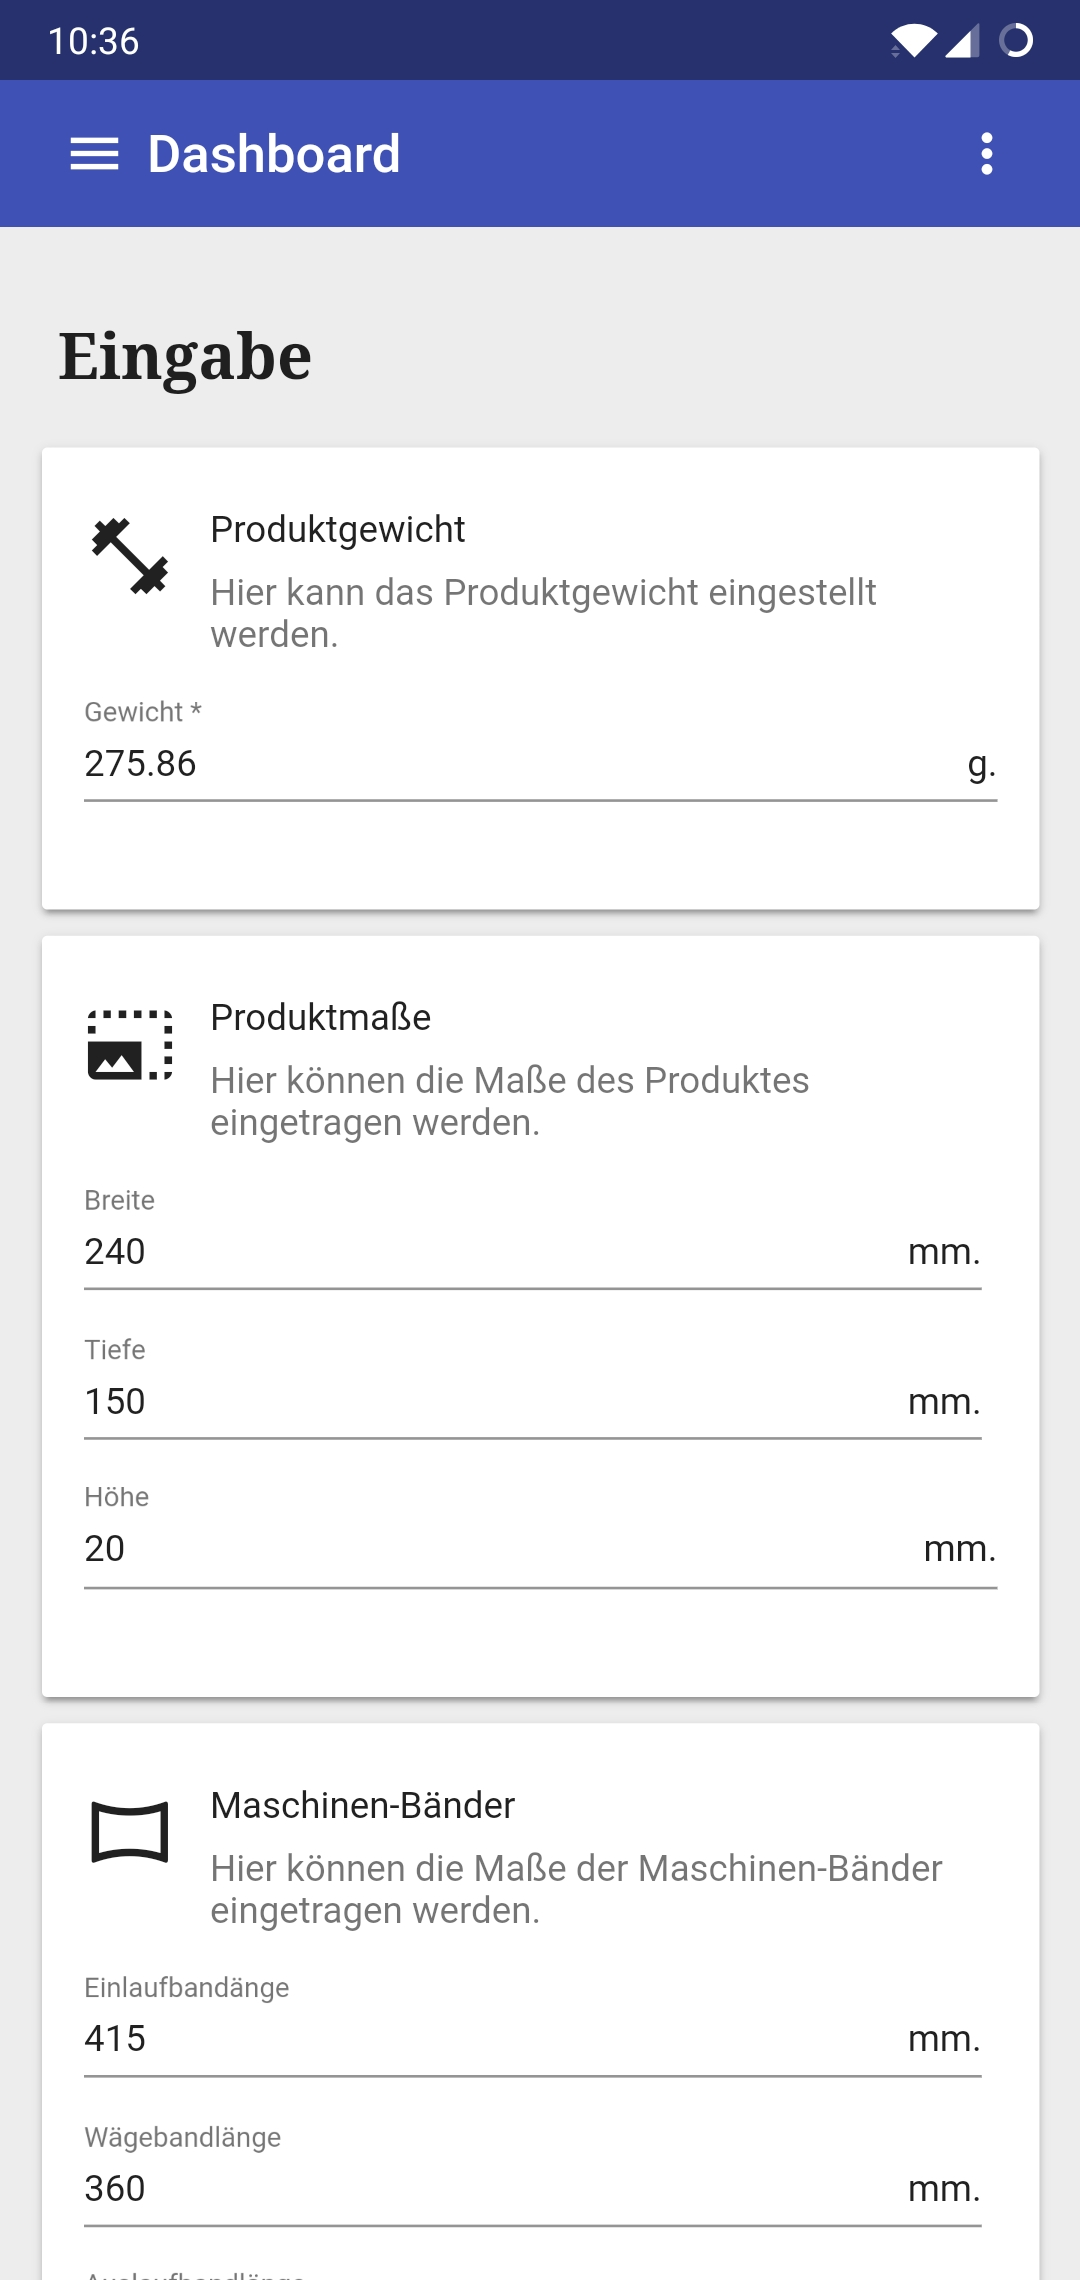
\includegraphics[scale=0.15]{images/kapitel_4/website_smartphone.jpg}
    \caption{Web-Frontend im Smartphone}
    \label{fig:umsetzung_website_smartphone}
\end{figure}

%% TODO noch schreiben
\subsubsection{Service Worker}
Der wird eingerichtet...
\colorbox{yellow}{Hier fehlt was}

%% TODO noch schreiben
\subsubsection{Offline Mode}
Dann kann man alles speichern, damit es offline verfügbar ist.
\colorbox{yellow}{Hier fehlt was}

%% TODO noch schreiben
\subsubsection{Weitere Funktionalitäten}
Offline Modus -> Kein Request an API,
\colorbox{yellow}{Hier fehlt was}

%% TODO noch schreiben
\subsubsection{Toolchain einrichten}
\colorbox{yellow}{Hier fehlt was}

\begin{figure}[h]
    \centering
    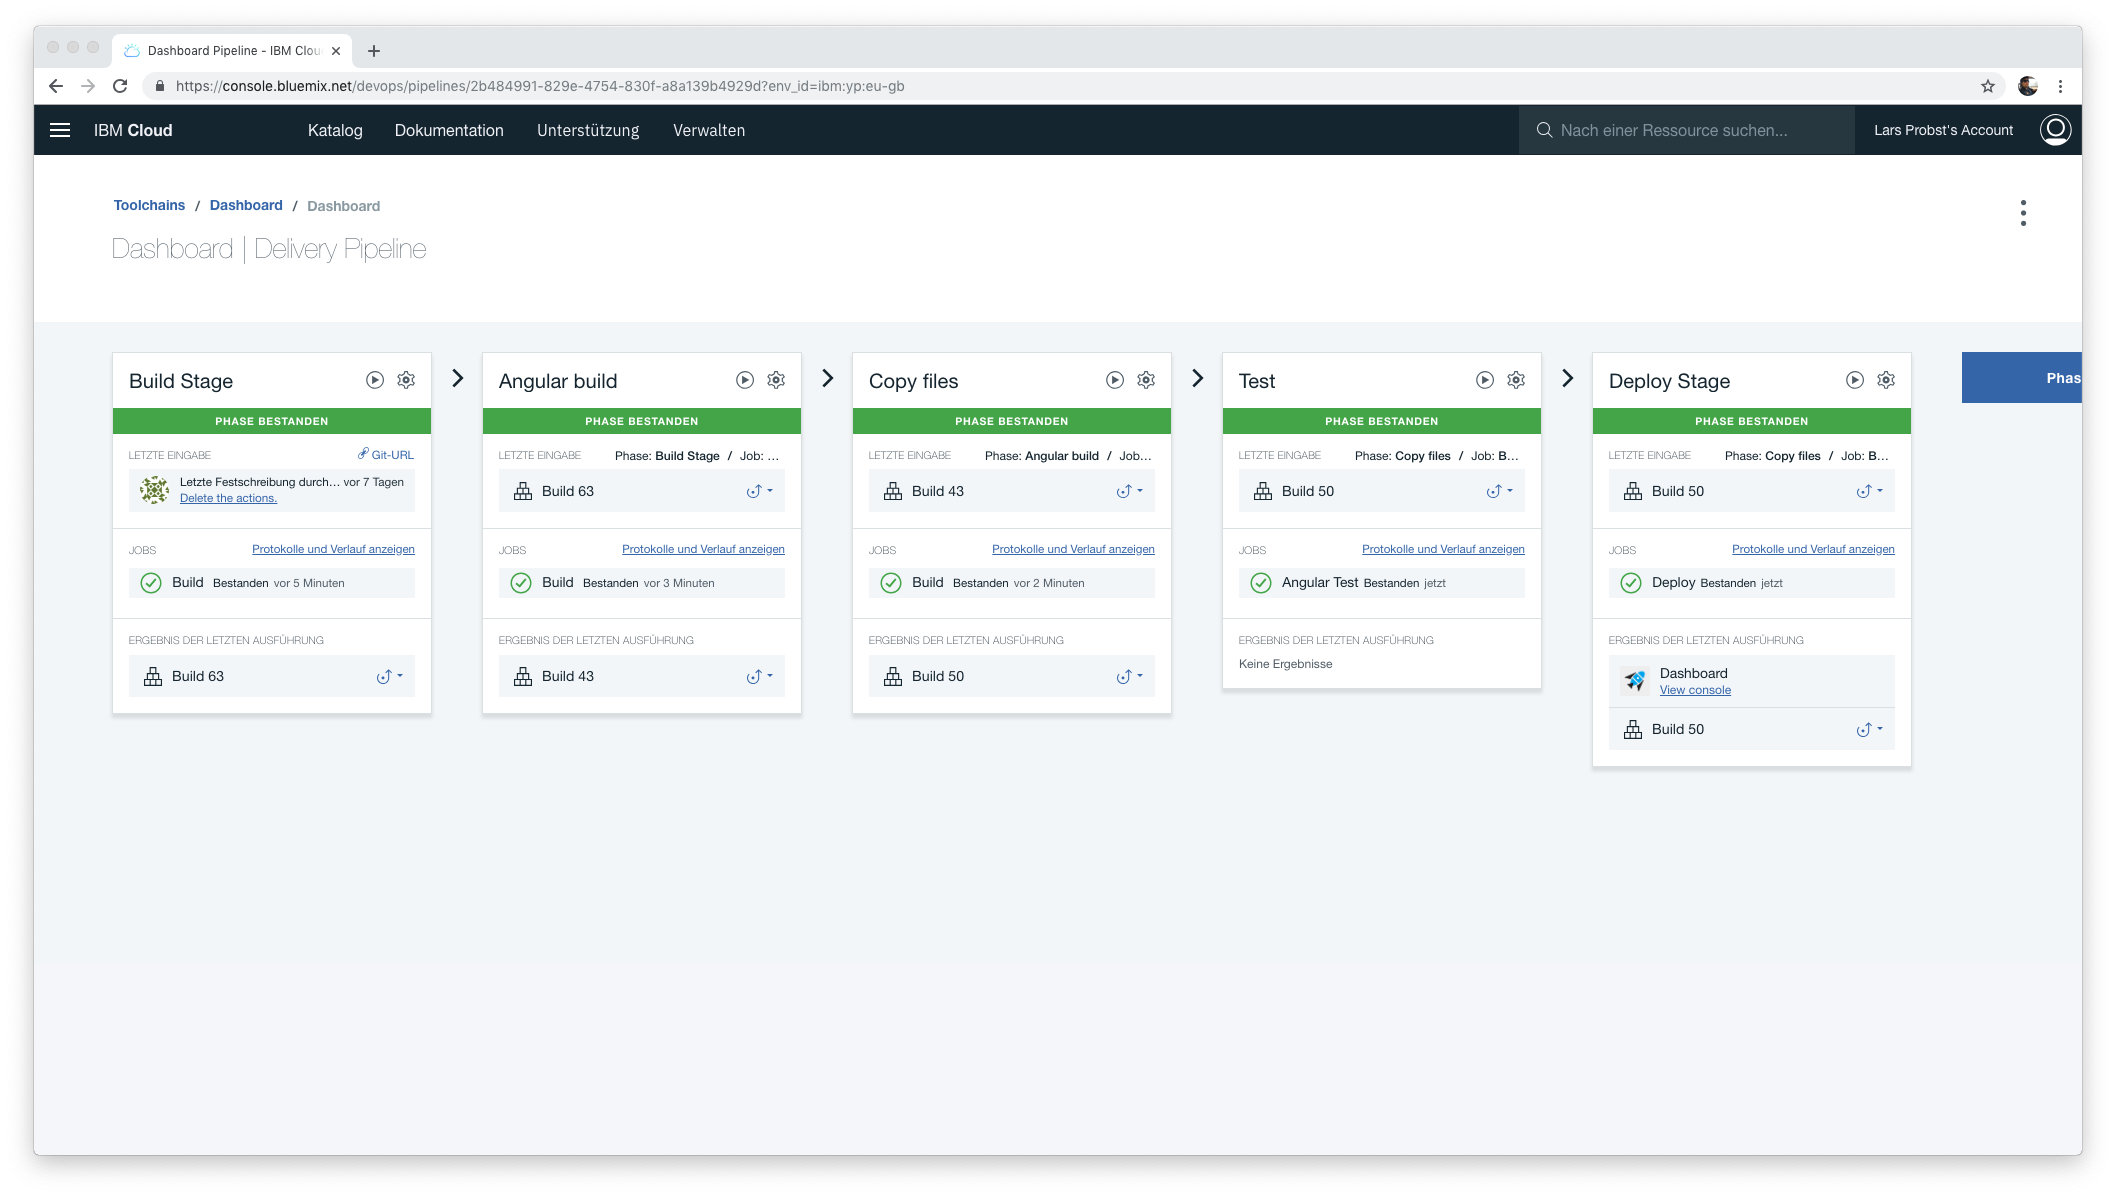
\includegraphics[width=\textwidth]{images/kapitel_4/toolchain_pipeline.png}
    \caption{Übersicht der Toolchain-Konfiguration}
    \label{fig:umsetzung_toolchain_pipeline_frontend}
\end{figure}

\subsection{Smartphone App}
Da das Frontend (Dashboard) nun fertig entwickelt ist, kann man es im nächsten Schritt für die Umsetzung der
Smartphone-App nutzen.

Die Umsetzung der Smartphone-App erfolgt auf Basis von Android und iOS. Dies hat den Vorteil, dass ein größerer
potentieller Kundenkreis gewonnen werden kann, da diese beiden Systeme die mobilen Betriebssysteme
dominieren~\cite{online_umsetzung_mobileos}.

In den zwei weiteren Kapiteln werden die Umsetzungen für die beiden Betriebssysteme erläutert. Insbesondere wird auf die
technischen Unterschiede der Systeme eingegangen.

%% TODO noch schreiben
\subsubsection{Android}
Bauen und erstellen der Apps

\colorbox{yellow}{Hier fehlt was}

\begin{figure}[h]
    \centering
    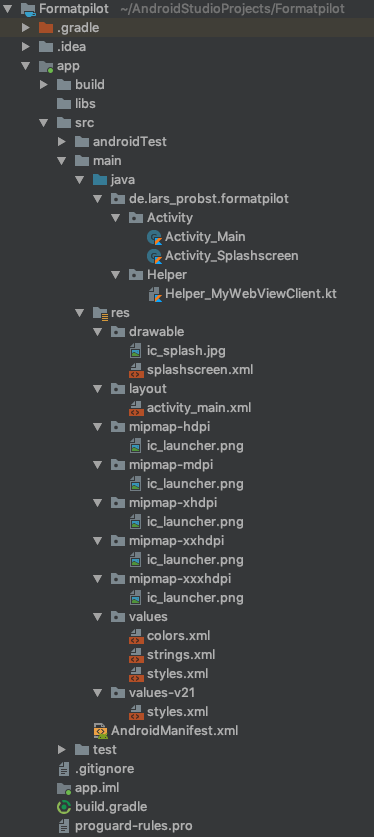
\includegraphics[scale=0.4]{images/kapitel_4/android_folder.png}
    \caption{Ordner und Dateien in Android Studio}
    \label{fig:umsetzung_android_folder}
\end{figure}

\begin{figure}[h]
    \centering
    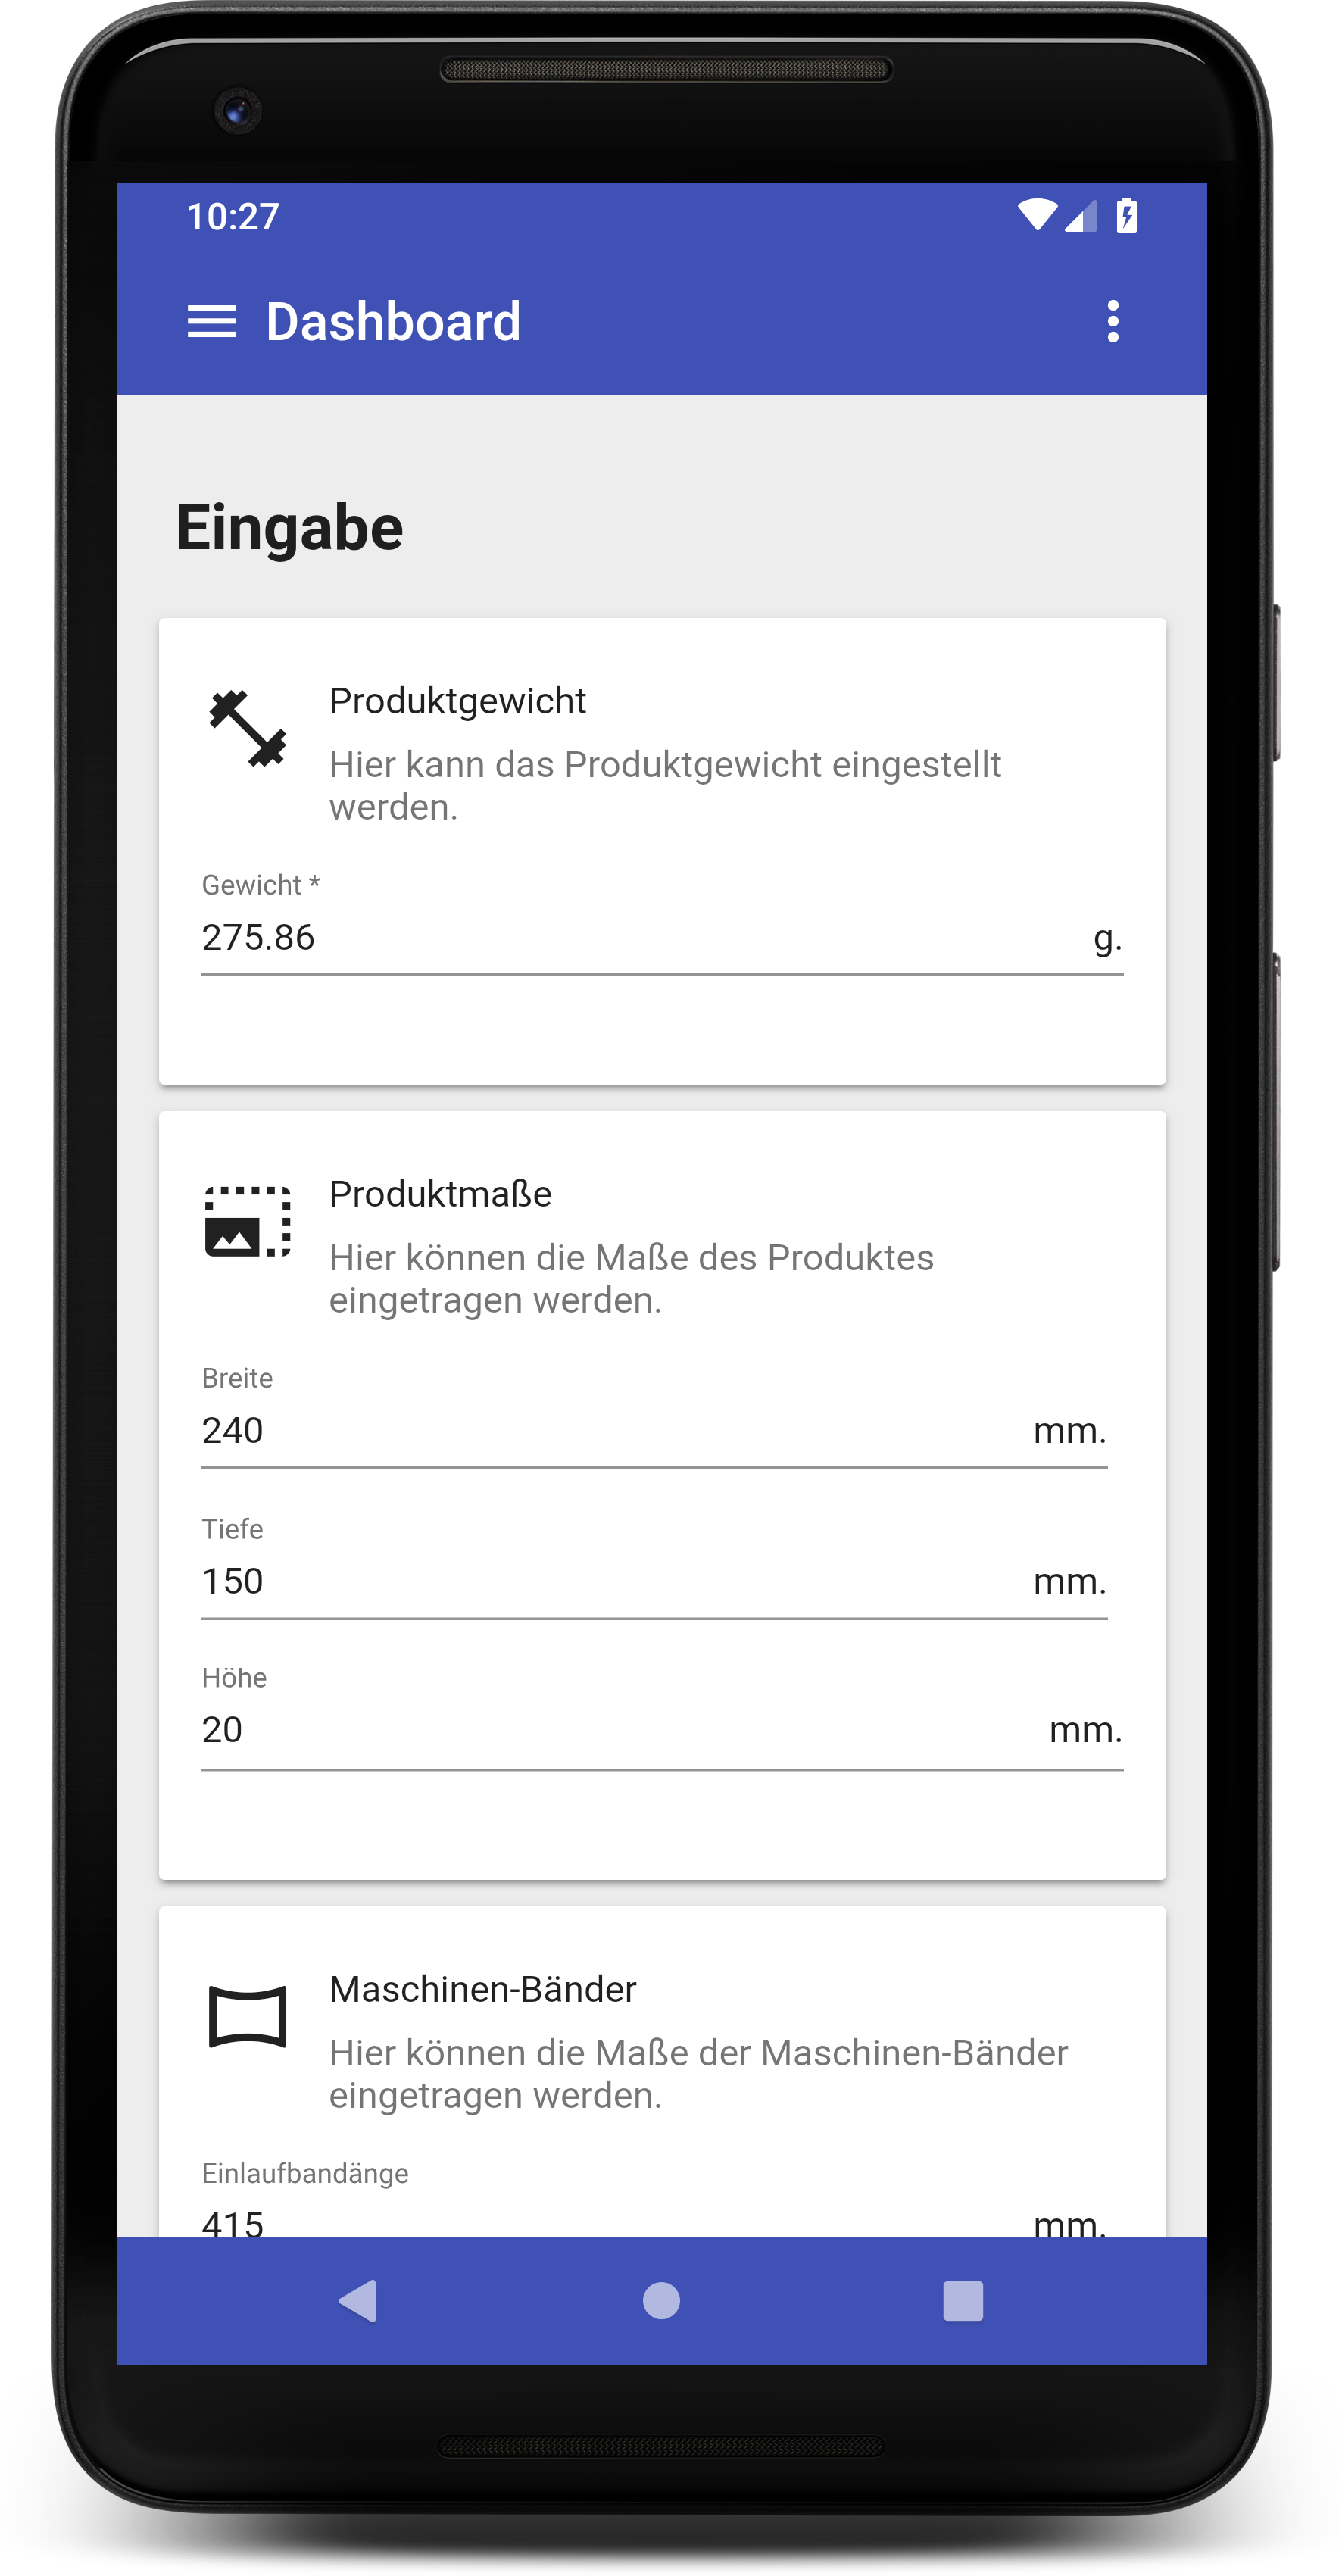
\includegraphics[scale=0.1]{images/kapitel_4/android_app.png}
    \caption{Android-App im Smartphone-Emulator}
    \label{fig:umsetzung_android_app}
\end{figure}

%% TODO noch schreiben
\subsubsection{iOS}
Bauen und erstellen der Apps

\colorbox{yellow}{Hier fehlt was}

\begin{figure}[h]
    \centering
    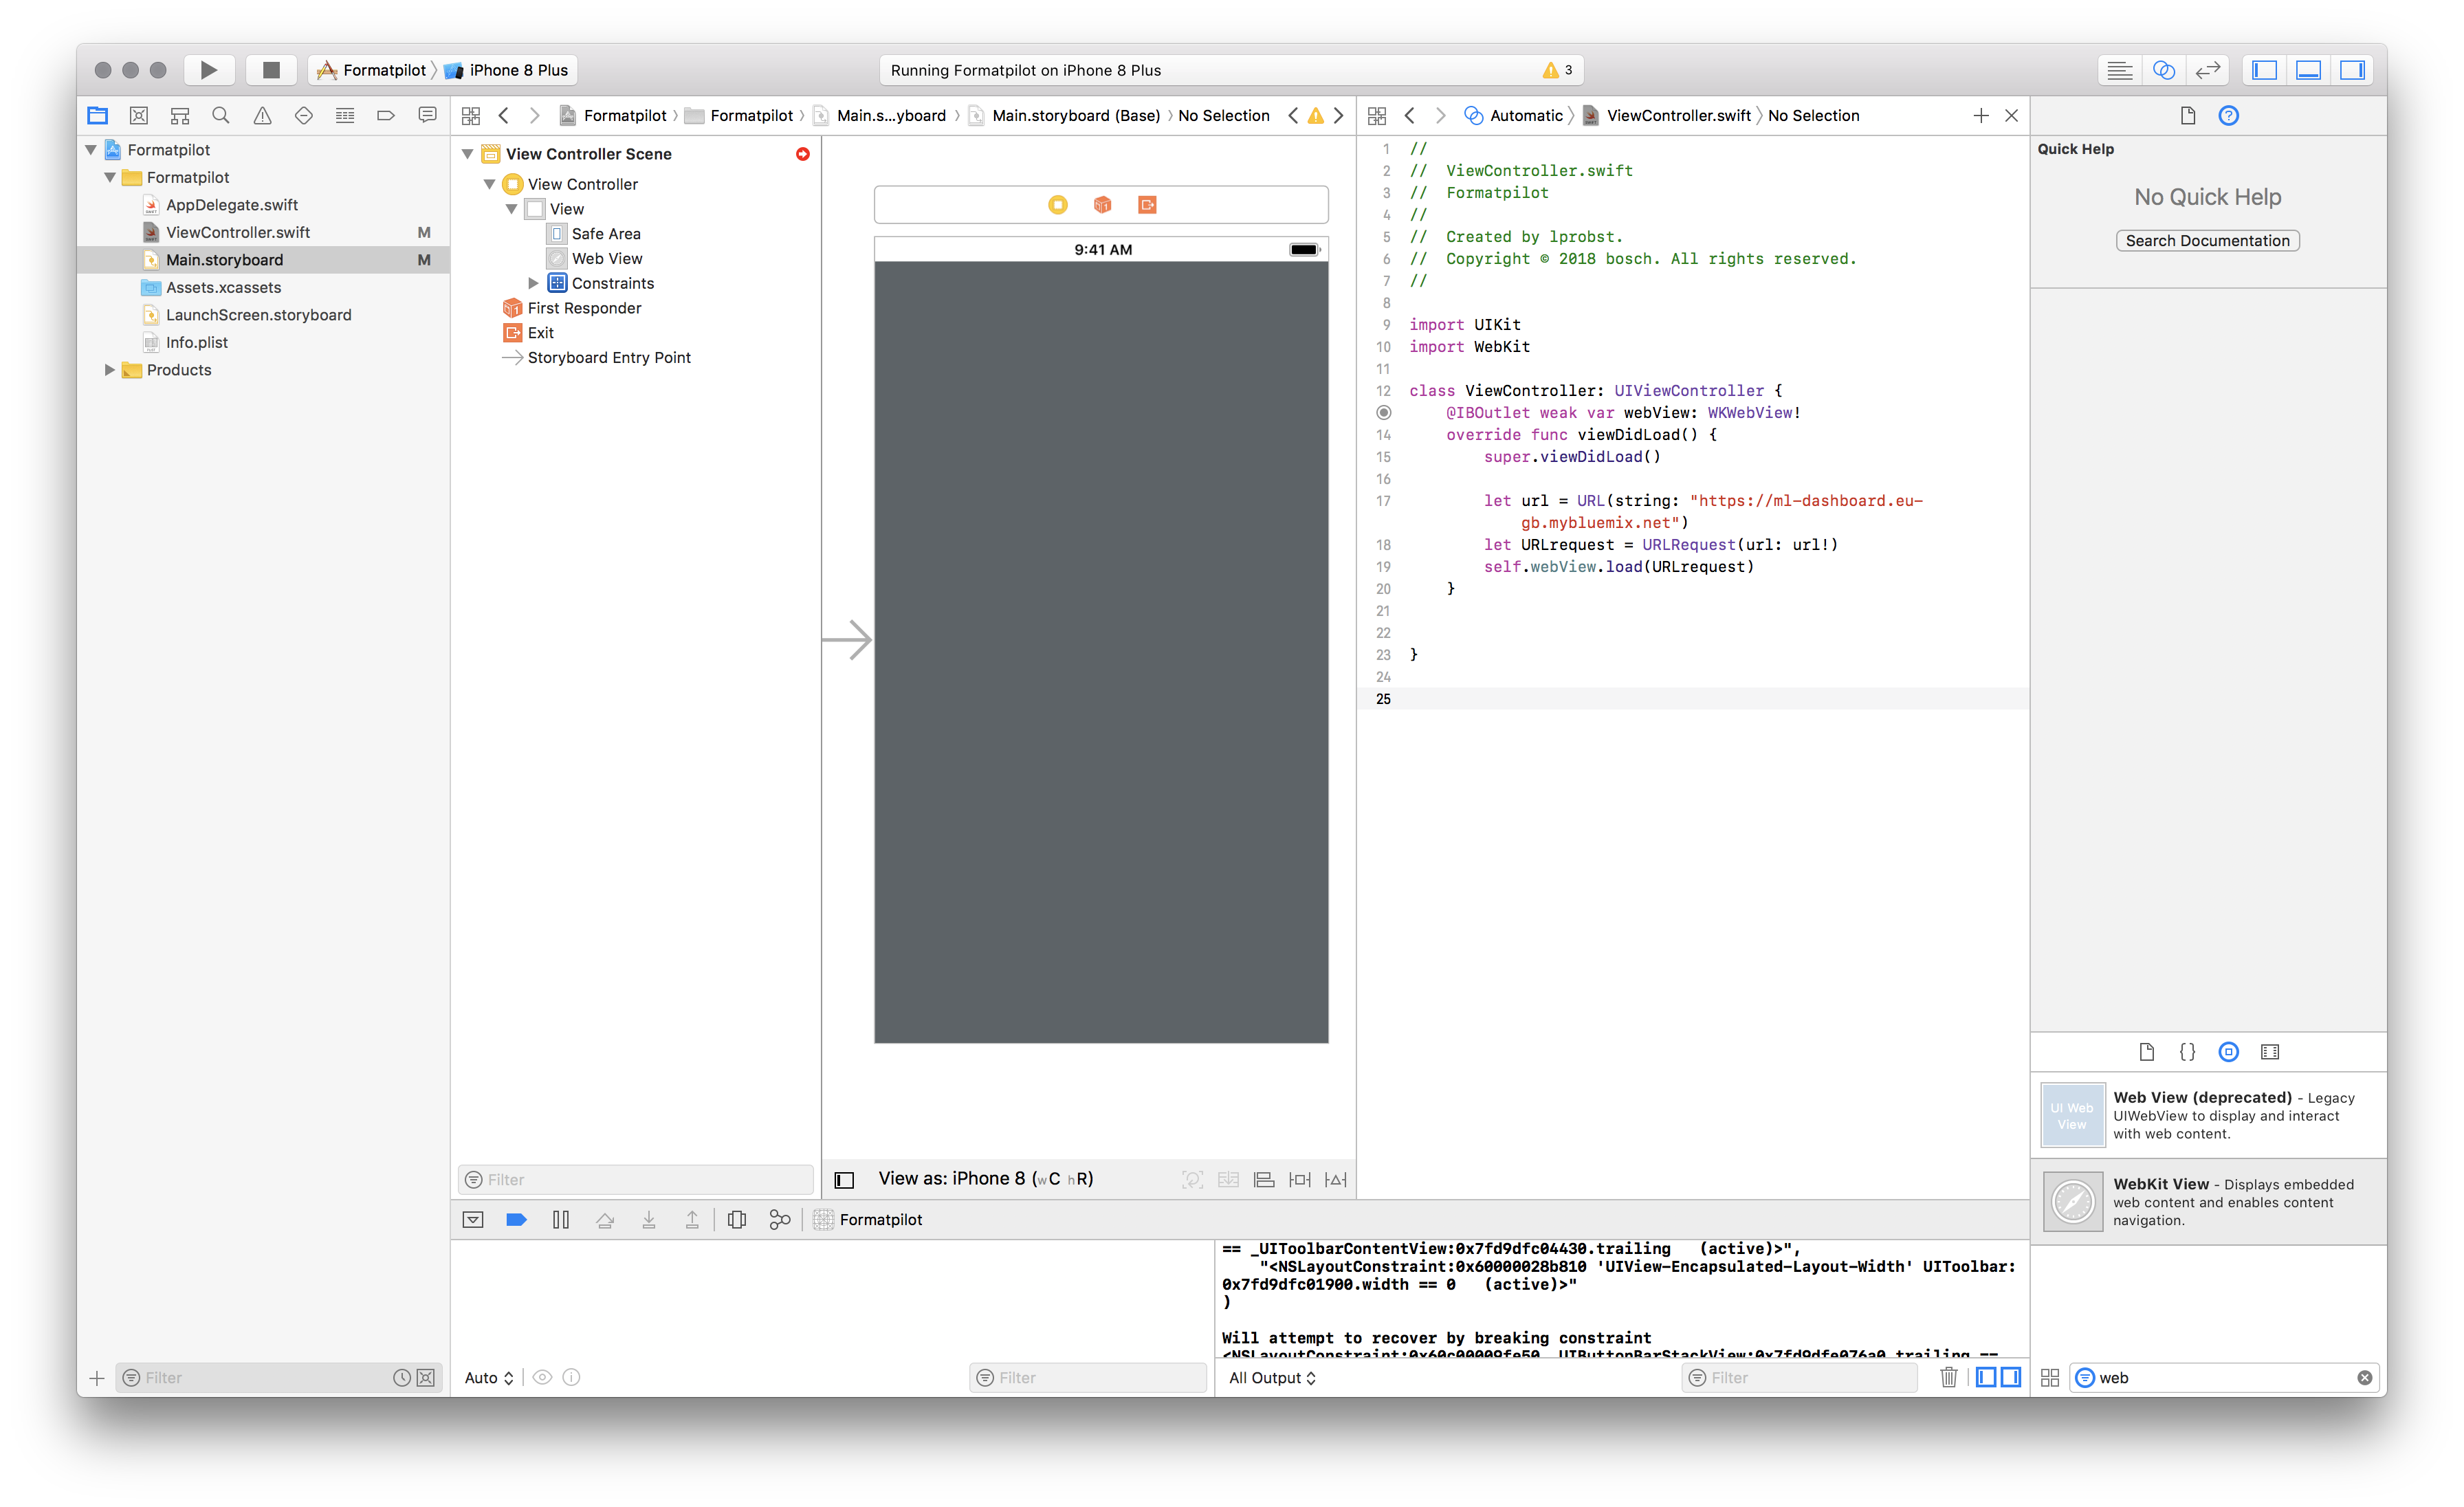
\includegraphics[width=\textwidth]{images/kapitel_4/ios_ide.png}
    \caption{Übersicht von xCode}
    \label{fig:umsetzung_ios_ide}
\end{figure}

\begin{figure}[h]
    \centering
    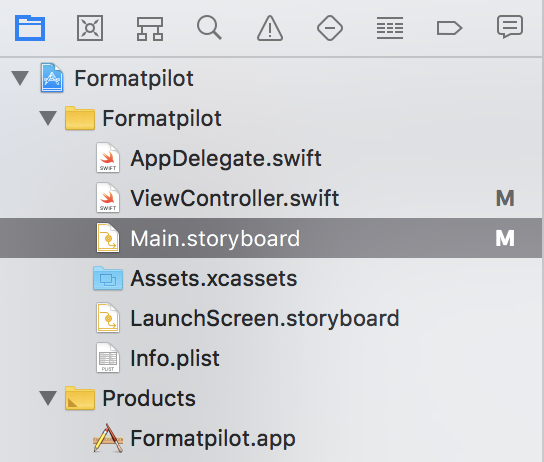
\includegraphics[scale=0.7]{images/kapitel_4/ios_folder.png}
    \caption{Ordner und Dateien in xCode}
    \label{fig:umsetzung_ios_folder}
\end{figure}

\begin{figure}[h]
    \centering
    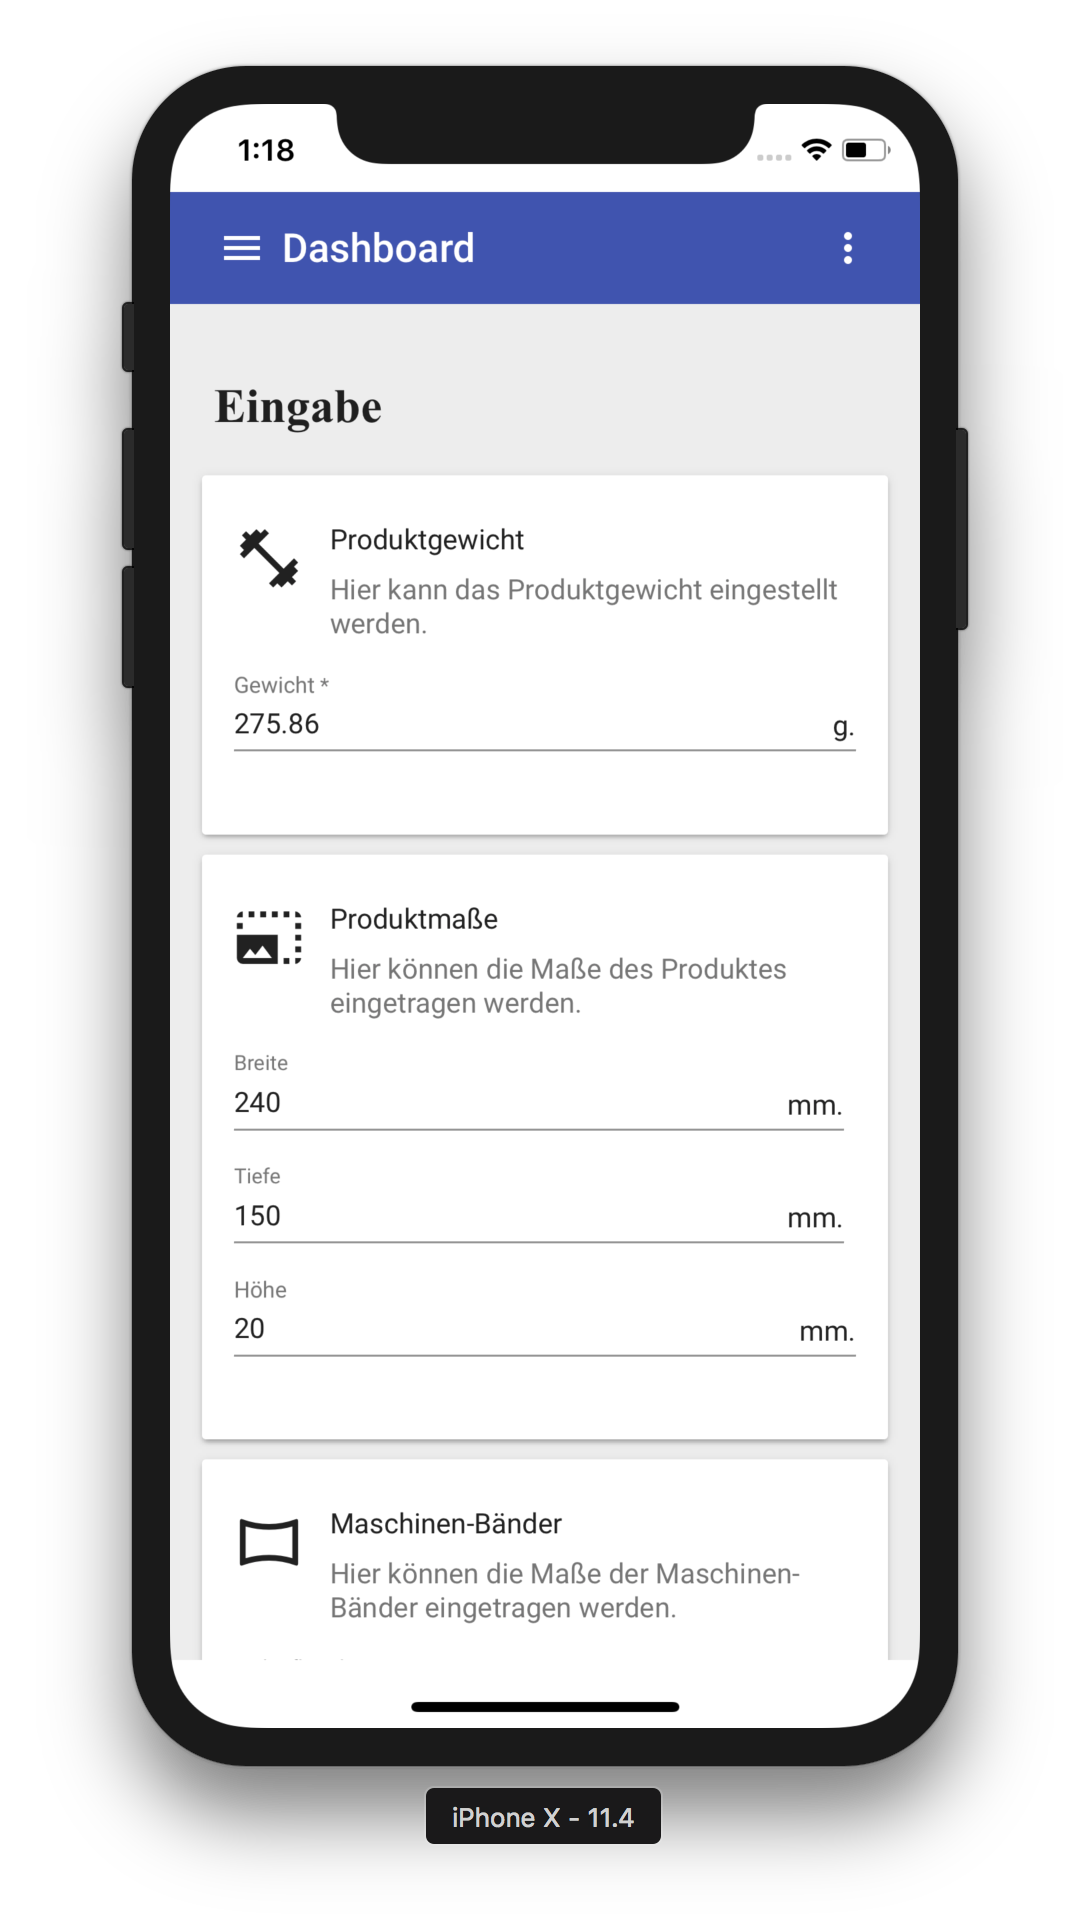
\includegraphics[scale=0.4]{images/kapitel_4/ios_app.png}
    \caption{iOS-App im Smartphone-Emulator}
    \label{fig:umsetzung_ios_app}
\end{figure}